\documentclass[a4paper]{article}

\usepackage[margin=2.5cm]{geometry}
\usepackage[pdftex]{graphicx}
\usepackage[utf8]{inputenc}
\usepackage[T1]{fontenc}
\usepackage{textcomp}
\usepackage{babel}
\usepackage{amsmath, amssymb}
\usepackage[colorlinks=true,linkcolor=blue]{hyperref}
\usepackage{float}
\usepackage{mathrsfs}
%\usepackage{enumitem}
%% for identity function 1:
\usepackage{bbm}
%%For category theory diagrams:
%\usepackage{tikz-cd}
%%For code (e.g. python) in latex:
%\usepackage{listings}
%
%Usage: 
%\begin{lstlisting}[language=Python]
%\end{lstlisting}

\newcommand{\incfig}[2][1]{%
\def\svgwidth{#1\columnwidth}
\import{./figures/}{#2.pdf_tex}
}


% figure support
\usepackage{import}
\usepackage{xifthen}
\pdfminorversion=7
\usepackage{pdfpages}
\usepackage{transparent}

\pdfsuppresswarningpagegroup=1

\setlength\parindent{0pt}

\newcommand{\qed}{\tag*{$\blacksquare$}}
\newcommand{\qedwhite}{\hfill \ensuremath{\Box}}

%Inequalities
\newcommand{\cycsum}{\sum_{\mathrm{cyc}}}
\newcommand{\symsum}{\sum_{\mathrm{sym}}}
\newcommand{\cycprod}{\prod_{\mathrm{cyc}}}
\newcommand{\symprod}{\prod_{\mathrm{sym}}}

%Linear Algebra

%Redeclaring Span and image
\DeclareMathOperator{\Span}{span}
\DeclareMathOperator{\Ima}{Im}
\DeclareMathOperator{\diag}{diag}
\DeclareMathOperator{\Ker}{Ker}
\DeclareMathOperator{\ob}{ob}


%Row operations
\newcommand{\elem}[1]{% elementary operations
\xrightarrow{\substack{#1}}%
}

\newcommand{\lelem}[1]{% elementary operations (left alignment)
\xrightarrow{\begin{subarray}{l}#1\end{subarray}}%
}

%SS
\DeclareMathOperator{\supp}{supp}
\DeclareMathOperator{\Var}{Var}

%NT
\DeclareMathOperator{\ord}{ord}

%Alg
\DeclareMathOperator{\Rad}{Rad}
\DeclareMathOperator{\Jac}{Jac}

\DeclareMathAlphabet{\pazocal}{OMS}{zplm}{m}{n}
\newcommand{\unif}{\pazocal{U}}

\begin{document}
\textbf{5.0.1:} Define the map $x \stackrel{f}{\to} \frac{x}{\|x\| + 1}$ for $x \in
    \mathbb{R}^{n}$, and $g  \colon (B^{n})^{\circ} \to \mathbb{R}^{n}$ the
    inclusion. Then
    $H  \colon \mathbb{R}^{n} \times I \to \mathbb{R}^{n}$ by
    \[
    H \left( x, t \right) = t f(x) + (1-t) x
    \] 
    gives the homotopy $g \circ f \simeq \mathbbm{1}_{\mathbb{R}^{n}}$ since
    $H(x,0) = \mathbbm{1}_{\mathbb{R}^{n}}$ while $H(x,1) = g \circ f$, and
    $H$ is continuous as $\mathbb{R}^{n}$ is convex.\\
    \linebreak
    Similarly, let
    $G  \colon B^{n \circ} \times I \to B^{n \circ} $ be given by
    \[
    G(x,t) = t f(x) + (1-t) x.
    \] 
    This is also a homotopy since
    $G(x,0) = \mathbbm{1}_{B^{n \circ}}$ and
    $G(x,1) = f \circ g$, and it is continuous since
    the set $B^{n \circ}$ is convex and at all times
    \[
    \|G(x,t)\| < 1
    \] 
    and is the linear homotopy connecting $x $ and $f(x)$.\\
    \linebreak
    \textbf{5.0.2:} We have that $\mathbb{R}P^{n}$ is the quotient of 
    $S^{n}$ by the antipodal map. This is equivalent to taking a hemisphere
    $D^{n}$ and identifying the antipodal points of  $\partial D^{n}$. But
    since
    $\partial D^{n}$ with antipodal points identified is 
    $\mathbb{R}P^{n-1}$, we have that $\mathbb{R}P^{n}$ is 
    just $\mathbb{R}P^{n-1}$ with an n-cell attached. By induction, we find
    that $\mathbb{R}P^{n}$ has a cell complex structure
    $e^{0} \cup e^{1} \cup \ldots \cup e^{n}$. 

    \begin{figure}[H]
        \centering
        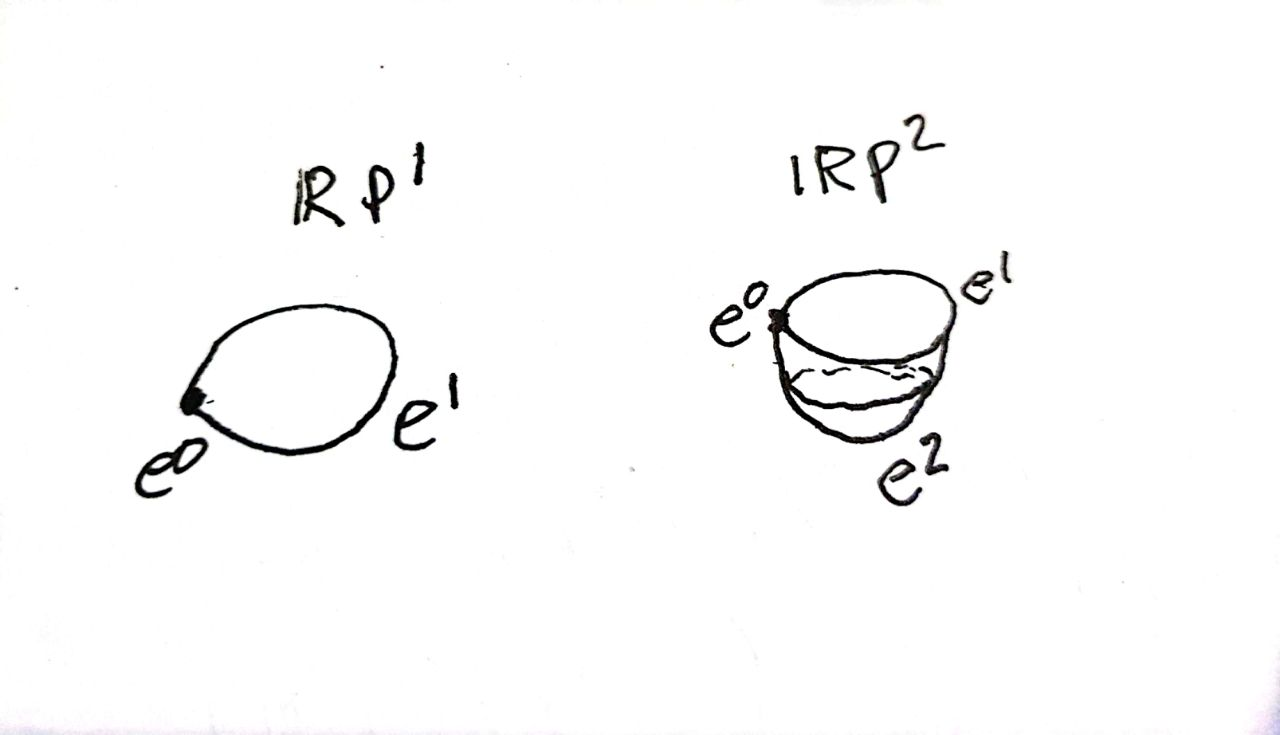
\includegraphics[width=0.8\textwidth]{2.jpg}
        \label{fig:2-jpg}
    \end{figure}
    
    
    
    






















\end{document}
